% !TEX encoding = UTF-8
% !TEX TS-program = pdflatex
% !TEX root = ../tesi.tex

%**************************************************************
\newgeometry{a4paper, left=30mm, right=30mm, top=5mm, bottom=30mm}

\chapter{Introduzione}
\label{cap:introduzione}
%**************************************************************

\noindent \intro{In questo capitolo si introduce brevemente l'azienda ospitante e il progetto affrontato.}\\

%Introduzione al contesto applicativo.\\

%\noindent Esempio di utilizzo di un termine nel glossario \\
%\gls{api}. \\

%\noindent Esempio di citazione in linea \\
%\cite{site:agile-manifesto}. \\

%\noindent Esempio di citazione nel pie' di pagina \\
%citazione\footcite{womak:lean-thinking} \\

%**************************************************************
\section{L'azienda}

\noindent{\myCompany} \cite{site:ergon-informatica}
(da qui in poi
\textit{"Ergon Informatica"}) è un'azienda italiana, fondata nel 1988, 
con sede a Castelfranco Veneto.\\
Essa si occupa principalmente di soluzioni gestionali per piccole e medie imprese e dello sviluppo di
\textit{software \gls{erpg}} (\textit{Enterprise Resource Planning}) per i settori dell'alimentare e dei trasporti,
ma completa l'offerta con la vendita di prodotti
\textit{hardware}, servizi \textit{web} e \textit{hosting}, nonché con progetti di \textit{\gls{serverconsolidationg}} e virtualizzazione di
sistemi.
L'azienda inoltre si è sviluppata in maniera costante negli anni e oggi può vantare una posizione di tutto rispetto tra le aziende dello stesso settore.
Attualmente fanno parte della stessa gestione:

\begin{itemize}
    \item \textit{Ergon Informatica S.R.L.}: che si occupa del \textit{software};
    \item \textit{Ergon S.R.L.}: che si occupa dei servizi tecnologici;
    \item \textit{Ergon Servizi S.R.L.}: che si occupa dei servizi amministrativi, logistici e di \textit{marketing} delle altre due parti.
\end{itemize}
Il logo dell'azienda è illustrato in Figura \ref{fig:logo}.
\vfill
\begin{figure}[!h]
    \centering
    
\includegraphics[width=0.8\columnwidth]{loghi/Ergon_Logo.pdf}
    \caption{Logo \myCompany}
    \label{fig:logo}
\end{figure}
\vfill
\noindent Il prodotto di proprietà dell'azienda è \textit{\gls{ergdisg}}, sistema \textit{\gls{erpg}}
il cui insieme dei moduli copre ogni aspetto della conduzione aziendale.
Alcuni di essi, inoltre, si possono interfacciare con dispositivi automatici presenti in azienda, come, ad esempio,
linee di confezionamento o \textit{robot}.

\newgeometry{a4paper, left=30mm, right=30mm, top=31mm, bottom=30mm}
\newpage
\noindent In particolare  vengono gestiti compiti che si dislocano in vari ambiti e
i moduli vengono dunque raggruppati nelle seguenti categorie:
\begin{multicols}{2}
\begin{itemize}
    \item Amministrazione e Finanza
    \item Controllo di Gestione
    \item Area Acquisti
    \item Logistica
    \item Vendite
    \item Produzione
\end{itemize}
\begin{itemize}
    \item \textit{Web}
    \item \textit{\gls{businessintelligenceg}}
    \item Qualità
    \item Gestione Archivi e Documentazione
    \item Pianificazione Consegne
    \item Area \textit{Mobile}
\end{itemize}
\end{multicols}

\noindent In generale, l'azienda può contare su una vasta gamma di clienti,
in quanto i prodotti vengono sviluppati in base alle esigenze di ognuno di essi.
Il prodotto viene prima creato a partire da uno \textit{standard}
a cui vengono successivamente aggiunte le varie funzionalità.\\
Il fatto di poter creare dei prodotti \textit{custom}, rende l'azienda altamente competitiva
e proprio per questo motivo il contatto
continuo con gli \textit{\gls{stakeholdersg}} è molto importante sia per accontentare le loro richieste che per
far evolvere \textit{\gls{ergdisg}} in una maniera tale da essere sempre in linea con le esigenze di mercato.


%**************************************************************
\section{L'idea dello stage}
\noindent Lo \textit{stage} proposto consiste nella progettazione e nello sviluppo di un modulo \textit{software} volto
ad assistere l'azienda nella fase di approvvigionamento dei prodotti dai propri fornitori, supportandola nello scegliere
da quale fornitore e quando acquistare i prodotti.
\noindent Questa nuova funzionalità andrebbe ad ottimizzare un modulo già esistente facente parte della
gestione dell'\textit{Area Acquisti}.\\
In pratica il modulo attuale, per ogni prodotto da ordinare, prende in considerazione l'ultima data d'ordine disponibile prima dell'inizio
dell'effettiva copertura del fabbisogno del prodotto stesso. Questo dunque non garantirebbe con certezza una scelta ottimale
in relazione alle possibilità d'ordine fornite dagli appositi listini e calendario dei fornitori.\\

\noindent Data la natura combinatoria del problema, che richiede di scegliere il mix migliore di acquisti da vari listini, il nuovo modulo dovrà fornire in tempi ragionevoli una "buona soluzione"
del problema, ovvero tendente il più possibile all'ottimo, e dovrà integrarsi con l'intero sistema \textit{\gls{ergdisg}}.\\

\noindent È previsto inoltre che i dati su cui si è eseguita l'ottimizzazione e il confronto dei risultati vengano visualizzati tramite un'apposita
interfaccia grafica che verrà sviluppata in linea con l'ambiente di sviluppo dell'azienda (\textit{\gls{.netg}} e \textit{\gls{devexpressg}}).


%**************************************************************
\section{Descrizione dello \textit{stage}}

%**************************************************************
\subsection{Introduzione}
\label{sec:descrizione-stage-intro}

\noindent Lo \textit{stage} consiste nello sviluppo di un algoritmo di ottimizzazione che riesca a diminuire la spesa dell'azienda per gli approvviogionamenti.\\
L'algoritmo dovrà ottimizzare i risultati calcolati da un modulo preesistente, facente parte della gestione dell'\textit{Area Acquisti}, il quale
consiglia di procedere con gli acquisti con una priorità basata sull'ultima data d'ordine disponibile.\\
\noindent La scelta dell'attuale modulo infatti porterebbe a non considerare:
\begin{itemize}
    \item \textbf{l'andamento del mercato}: i prezzi sono variabili e dipendono dal periodo nel quale si comprano i prodotti;
    \item \textbf{i bonus}: i fornitori possono garantire dei bonus in base al raggiungimento di determinati obiettivi di rapporti commerciali.
\end{itemize}
\noindent Facciamo un esempio per chiarire in maniera esplicita perchè si devono andare a considerare parametri come questi. Il problema
è molto semplificato e verrà discusso nei capitoli successivi.\\

%comando arraystretch
\renewcommand{\arraystretch}{1.2}

\begin{table}[!h]
    \begin{center}
        \begin{tabular}{c c c c}
            Articolo & Quantità & Data inizio copertura & Data fine copertura\\
            FEG10 & 2 & 01/07/2022 & 07/07/2022\\
            FRE02 & 3 & 06/07/2022 & 07/07/2022\\
        \end{tabular}
        \vspace{0.3cm}
        \caption{Esempio - Fabbisogni}
    \end{center}
\end{table}
\begin{table}[!h]
        \begin{center}
            \begin{tabular}{c c c c c}
                Articolo & Fornitore & Data inizio validità & Data fine validità & Prezzo(€)\\
                FEG10 & 47040 & 15/06/2022 & 21/06/2022 & 9.50\\
                FRE02 & 47040 & 15/06/2022 & 21/06/2022 & 10.00\\
                FEG10 & 46613 & 22/06/2022 & 31/12/9999 & 10.00\\
                FRE02 & 46613 & 22/06/2022 & 31/12/9999 & 9.50
            \end{tabular}
            \vspace{0.3cm}
            \caption{Esempio - Listino Prezzi}
        \end{center}
\end{table}
\begin{table}[!h]
    \begin{center}
        \begin{tabular}{c c c c}
            Articolo & Fornitore & Data spedizione & Data di arrivo\\
            FEG10 & 47040 & 17/06/2022 & 17/06/2022\\
            FRE02 & 47040 & 19/06/2022 & 19/06/2022\\
            FEG10 & 46613 & 31/06/2022 & 31/06/2022\\
            FRE02 & 46613 & 03/07/2022 & 03/07/2022\\
        \end{tabular}
        \vspace{0.3cm}
        \caption{Esempio - Calendario spedizioni}
    \end{center}
\end{table}

\noindent Il modulo attuale avrebbe sicuramente ordinato entrambi gli articoli dal fornitore \textit{46613},
per un totale di 48.50€. Tuttavia è evidente che non è la soluzione ottima.
Infatti sarrebbe stato opportuno ordinare l'articolo \textit{FEG10} dal fornitore \textit{47040} e il
\textit{FRE02} dal fornitore \textit{46613}, ottenendo dunque un totale di 47.50€.\\
Sebbene possa sembrare un risparmio minimo e trascurabile, se applicato a enormi quantità, può
diventare un notevole risparmio di risorse.\\

\noindent Dopo queste considerazioni, è chiaro come il modulo preesistente non garantisca necessariamente una soluzione ottima in termini economici ed è il motivo per il quale
si è deciso di realizzare un nuovo modulo.\\

\noindent Inoltre, i risultati devono poter essere visualizzati tramite una \textit{\gls{windowsformg}} in cui si dovrà far scegliere all'utente
anche le date entro cui si vuole fare l'analisi.\\

\noindent Per l'azienda, lo \textit{stage} di cui si riporta in questa tesi rappresenta un'opportunità per fornire un servizio aggiuntivo ai propri clienti, ma serve anche per avere una base
dalla quale poter eventualmente estendere il modulo con nuovi algoritmi più efficienti.
%**************************************************************
\newpage
\subsection{Obiettivi}
\label{sec:obiettivi}
\noindent Nella Tabella \ref{tab:obiettivi} vengono elencati tutti gli obiettivi previsti dallo \textit{stage} dove
i codici obiettivo con prefisso \textit{OB} rappresentano gli obiettivi obbligatori, \textit{DE} quelli desiderabili
e \textit{FA} quelli facoltativi.

\renewcommand{\arraystretch}{1.55}

% tabella con i risultati
\begin{center}
    \begin{longtable}{m{3cm}m{9cm}}
    \caption{Tabella degli obiettivi}
    \label{tab:obiettivi}
    \\ \hline
    \centering \textbf{Codice Obiettivo} & \centering \textbf{Descrizione Obiettivo} \arraybackslash \\
    \hline
    \centering OB1 & Sviluppo programmi per inserimento
    dei vincoli che delimitano il problema \arraybackslash \\
    \hline
    \centering OB2 & Redazione di un documento che riporti
    i risultati ottenuti nello studio di fattibilità \arraybackslash \\
    \hline
    \centering OB3 & Sviluppo di micro-moduli di prototipizzazione degli algoritmi analizzati \arraybackslash \\
    \hline
    \centering OB4 & Sviluppo modulo \textit{software} per
    la soluzione del problema \arraybackslash \\
    \hline
    \centering OB5 & Acquisizione di competenze sull’utilizzo
    di algoritmi di \gls{ricercaoperativag} e
    applicazione in un caso reale \arraybackslash \\
    \hline
    \centering DE1 & Utilizzo di più tecniche e combinazione dei risultati
    ottenuti o individuazione della miglior soluzione attraverso
    opportuni \textit{KPI} (\textit{Key Performance Indicator}) \arraybackslash \\
    \hline
    \centering FA1 & Utilizzo del \textit{multithreading}
    nelle fasi in cui è richiesta una
    maggiore capacità di calcolo \arraybackslash \\
    \hline
    \end{longtable}
\end{center}%

\subsection{Pianificazione del lavoro}
\label{sec:pianificazione-lavoro}
\noindent Lo stage è stato programmato per essere svolto in due mesi di lavoro
a tempo pieno, per un totale di 320 ore (festività escluse).\\
\noindent Nella Tabella \ref{tab:attivita-ore-inizio} vengono elencate
le attività preventivate con le corrispettive ore.

\renewcommand{\arraystretch}{1.55}

% tabella con i risultati
\begin{center}
    \begin{longtable}{m{9cm}m{3cm}}
    \caption{Tabella delle attività con le corrispettive ore preventivate}
    \label{tab:attivita-ore-inizio}
    \\ \hline
    \centering \textbf{Descrizione attività} & \centering \textbf{Ore preventivate} \arraybackslash \\
    \hline
    \centering Analisi del modulo \textit{software}
    esistente e delle funzionalità da realizzare & \centering 24 \arraybackslash \\
    \hline
    \centering Studio di fattibilità e Studio di algoritmi e tecniche di
    \gls{ricercaoperativag}
    e Ottimizzazione Combinatoria & \centering 100 \arraybackslash \\
    \hline
    \centering Studio delle tecnologie aziendali necessarie allo sviluppo del
    modulo & \centering 32 \arraybackslash \\
    \hline
    \centering Sviluppo di micro-moduli di \textit{test} per gli algoritmi
    studiati & \centering 8 \arraybackslash \\
    \hline
    \centering Sviluppo modulo effettivo, generazione/lettura dei vincoli
    e parametrizzazione tramite pesi delle variabili & \centering 92 \arraybackslash \\
    \hline
    \centering \textit{Test} e Validazione & \centering 20 \arraybackslash \\
    \hline
    \centering Stesura della documentazione
    del prodotto sviluppato & \centering 24 \arraybackslash \\
    \hline
    \end{longtable}
\end{center}%

\newpage

\noindent In Figura \ref{gantt-diagramma} viene presentata
la pianificazione settimanale delle attività comprese tra
l'11/07/2022 e il 05/09/2022.
\begin{figure}[!h]
    \centering
    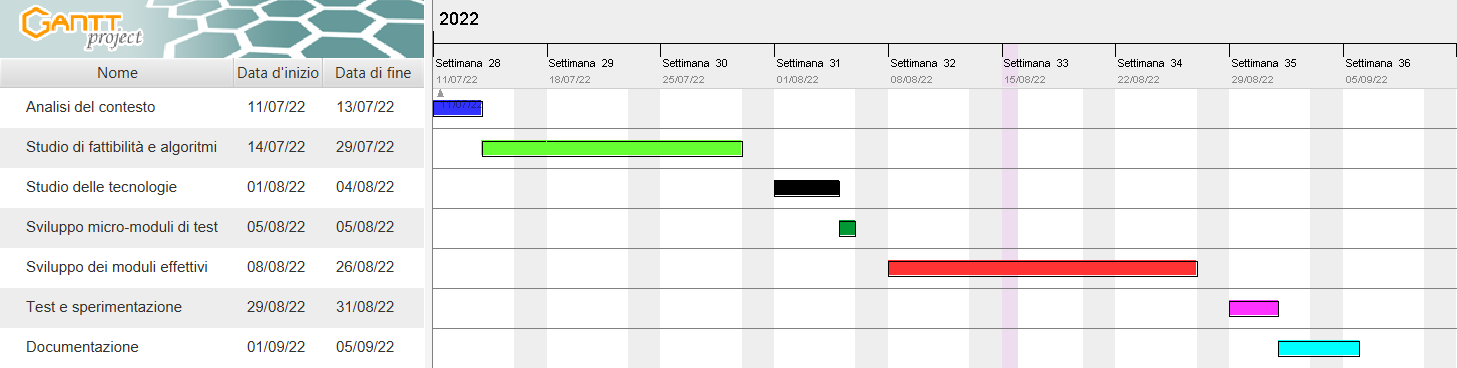
\includegraphics[width=0.95\columnwidth]{ganttdiagrams/Gantt Stage Ergon.png}
    \caption{Diagramma di Gantt delle attività}
    \label{gantt-diagramma}
\end{figure}

%**************************************************************
\subsection{Analisi preventiva dei rischi}
\noindent Durante la fase iniziale dello \textit{stage}, sono stati rilevati dei possibili rischi che avrebbero potuto presentarsi
durante il percorso del progetto.\\
Si sono dunque trovate delle soluzioni che potessero arginare i problemi. In particolare:
\begin{enumerate}
    \item \textbf{Comprensione e confronto degli algoritmi}\\[0.2cm]
    \textbf{Problema:} il progetto richiede un'ampia fase di studio che riguarda principalmente la teoria
    delle tecniche per la risoluzione di problemi di \gls{ricercaoperativag} e Ottimizzazione Combinatoria.
    Questo può portare la possibilità di non comprendere fino in fondo l'algoritmo e può essere difficile cogliere e confrontare
    i pregi e difetti di ciascuno di essi.\\[0.2cm]
    \textbf{Soluzione:} è stato organizzato un incontro iniziale con il \textit{tutor}
    per fornire una base da cui poi iniziare una ricerca più approfondita.
    Sono state fornite anche delle dispense utili per rafforzare la base di partenza.
    \item \textbf{Tecnologie e ambiente di sviluppo}\\[0.2cm]
    \textbf{Problema:} sono richieste alcune tecnologie, come per esempio \textit{\gls{entityframeworkg}} o
    \textit{\gls{devexpressg}} a me assolutamente ignote.
    Sebbene avessi delle basi abbastanza solide di \textit{C\#} derivanti dalla conoscenza di altri linguaggi
    quali \textit{\gls{C++g}} e \textit{\gls{javag}}, venivano richieste tuttavia
    alcune tecnologie integrate nel linguaggio, come per esempio le \textit{\gls{linqg}} (\textit{Language-Integrated Query}), anch'esse ignote. L'ambiente di sviluppo e
    l'\textit{\gls{ideg}} non erano mai stati utilizzati.\\[0.2cm]
    \textbf{Soluzione:} sono stati forniti dei riferimenti consigliati per l'autoapprendimento.
    Tuttavia qualsiasi dubbio ulteriore
    poteva essere richiesto al \textit{tutor}. È stato effettuato insieme al \textit{tutor} il \textit{setup} dell'ambiente di sviluppo e la conseguente creazione dei \textit{\gls{databaseg}}.
    \item \textbf{Calibrazione dei parametri e funzione di valutazione}\\[0.2cm]
    \textbf{Problema:} dopo la scelta e l'implementazione dell'algoritmo, è molto importante:
    \begin{itemize}
        \item definire una funzione di valutazione che vada a descrivere in maniera "buona" l'andamento dell'algoritmo stesso;
        \item calibrare i parametri in base allo spazio delle soluzioni del problema preso in esame.
    \end{itemize}
    Entrambe sono azioni molto delicate che possono compromettere il funzionamento stesso dell'algoritmo anche
    se implementato correttamente.\\[0.2cm]
    \textbf{Soluzione:} cercare una costruzione e calibrazione per passi e presentarle in una discussione con il \textit{tutor},
    in modo tale da creare una \textit{baseline} su cui basarsi per continuare con i passi successivi.

\end{enumerate}

\noindent
%**************************************************************
\section{Organizzazione del testo}
\noindent Di seguito viene illustrata l'organizzazione dei capitoli successivi:
\begin{description}
    \item[{\hyperref[cap:studio-fattibilita]{Il secondo capitolo}}] 
    approfondice lo studio di fattibilità effettuato, utile per entrare a conoscenza
    delle più utilizzate tecniche di ottimizzazione combinatoria e per analizzare
    quali siano i vantaggi e svantaggi di ognuno di essi.
    
    \item[{\hyperref[cap:analisi-requisiti]{Il terzo capitolo}}]
    descrive l'analisi dei requisiti del progetto, comprensiva di diagrammi dei
    casi d'uso e raccolta dei requisiti derivanti dall'analisi di questi ultimi.
    
    \item[{\hyperref[cap:progettazione-codifica]{Il quarto capitolo}}]
    approfondisce le fasi di progettazione e codifica, comprensiva di diagrammi delle classi
    e di approfondimenti a livello implementativo.
    
    \item[{\hyperref[cap:verifica-validazione]{Il quinto capitolo}}]
    espone tutte le verifiche effettuate durante il progetto e la validazione
    finale a conferma dei requisiti inizialmente stilati nella fase di
    analisi dei requisiti.
    
    \item[{\hyperref[cap:conclusioni]{Il sesto capitolo}}]
    presenta le conclusioni tratte dallo \textit{stage}, comprensivo di conoscenze
    acquisite e considerazioni di carattere personale.
\end{description}